\documentclass{beamer}
\usetheme{Boadilla}

\usepackage{graphicx}
\usepackage{subcaption}
\usepackage{csvsimple}

% Change size of footnotes
\renewcommand{\footnotesize}{\fontsize{5pt}{5pt}\selectfont}
\title{Analysis of gene regulatory properties underlying trait pleiotropy}
\subtitle{Meeting GOLD 2022}
\author{Aitor Gonz\'alez}
\institute{Aix Marseille Univ, INSERM, TAGC}
\date{Oct. 19, 2022}

% Add section slide
\AtBeginSection[]
{
\begin{frame}
\frametitle{Table of Contents}
\tableofcontents[currentsection]
\end{frame}
}

\begin{document}

%%%%%%%%%%%%%%%%%%%%%%%%%%%%%%%%%%%%%%%%%%%%%%%%%%%%%%%%%%%%%%%%%%%%%%%%%%%%%%%%
\begin{frame}

\titlepage

\end{frame}


\section{Introduction} %%%%%%%%%%%%%%%%%%%%%%%%%%%%%%%%%%%%%%%%%%%%%%%%%%%%%%%%%%%%%%

%%%%%%%%%%%%%%%%%%%%%%%%%%%%%%%%%%%%%%%%%%%%%%%%%%%%%%%%%%%%%%%%%%%%%%%%%%%%%%%%
\begin{frame}
\frametitle{Genome-wide association studies (GWAS)}

\begin{itemize}
\item Genetic loci with higher frequency in individuals with a given disease
\item A very active field with many studies
\item Many genetic variants are involved in several phenotypes
\end{itemize}
%
\vfill
%
Limitations
%
\begin{itemize}
\item Correlation between variants, ie. LD
\item Which cell types are causal to the disease?
\item Over 90\% GWAS variants fall in non-coding regions
\end{itemize}
%
\vfill
%
These limitations can be partially addressed by looking at eQTLs in different tissues

\let\thefootnote\relax\footnotetext{Cano-Gamez et al. 2020. doi:10.3389/fgene.2020.00424}

\end{frame}

%%%%%%%%%%%%%%%%%%%%%%%%%%%%%%%%%%%%%%%%%%%%%%%%%%%%%%%%%%%%%%%%%%%%%%%%%%%%%%%%
\begin{frame}
\frametitle{Expression quantitative trait loci (eQTL)}

\begin{columns}
\begin{column}{0.5\textwidth}
    \begin{center}
\includegraphics[width=\textwidth]{/home/gonzalez/Repositories/gwas2eqtl_pleiotropy/presentation_gold2022_paris/fig/doi_10.3389_fgene.2020.00424_fig4a.jpg}
     \end{center}
\end{column}
\begin{column}{0.5\textwidth}

\end{column}
\end{columns}

\let\thefootnote\relax\footnotetext{Cano-Gamez et al. 2020. doi:10.3389/fgene.2020.00424}
\end{frame}

%%%%%%%%%%%%%%%%%%%%%%%%%%%%%%%%%%%%%%%%%%%%%%%%%%%%%%%%%%%%%%%%%%%%%%%%%%%%%%%%
\begin{frame}
\frametitle{Colocalisation analysis of GWAS and eQTL variants}

\begin{columns}
\begin{column}{0.5\textwidth}
    \begin{center}
\includegraphics[width=\textwidth]{/home/gonzalez/Repositories/gwas2eqtl_pleiotropy/presentation_gold2022_paris/fig/doi_10.3389_fgene.2020.00424_fig4a.jpg}
     \end{center}
\end{column}
\begin{column}{0.5\textwidth}
    \begin{center}
\includegraphics[width=\textwidth]{/home/gonzalez/Repositories/gwas2eqtl_pleiotropy/presentation_gold2022_paris/fig/doi_10.3389_fgene.2020.00424_fig4bc.png}
     \end{center}
\end{column}
\end{columns}

\let\thefootnote\relax\footnotetext{Cano-Gamez et al. 2020. doi:10.3389/fgene.2020.00424}
\end{frame}

%%%%%%%%%%%%%%%%%%%%%%%%%%%%%%%%%%%%%%%%%%%%%%%%%%%%%%%%%%%%%%%%%%%%%%%%%%%%%%%%
\begin{frame}
\frametitle{Objectives}

\begin{enumerate}
\item Large scale colocalization analysis between GWAS and eQTL variants
\item To identify pleiotropic genetic loci
\item To characterize the regulatory causes of trait pleiotropy
\end{enumerate}
\end{frame}

%%%%%%%%%%%%%%%%%%%%%%%%%%%%%%%%%%%%%%%%%%%%%%%%%%%%%%%%%%%%%%%%%%%%%%%%%%%%%%%%
\begin{frame}
\frametitle{Data and Algorithms}

\begin{columns}
\begin{column}{0.5\textwidth}
\begin{itemize}
\item IEA OpenGWAS database$^1$: 244,881e6 associations from 42e3 GWAS datasets
\item EBI eQTLs database$^2$: Processed gene expression and splicing QTLs from all public studies on human.
\item CRAN - Package coloc$^3$: Genetic colocalisation analysis of two phenotypes to look for shared common genetic causal variants
\end{itemize}
\end{column}
\begin{column}{0.5\textwidth}
\begin{center}
\includegraphics[width=\textwidth]{/home/gonzalez/Repositories/gwas2eqtl_pleiotropy/presentation_gold2022_paris/fig/pgen.1004383.g001.png}
\end{center}
\end{column}
\end{columns}

\let\thefootnote\relax\footnotetext{$^1$https://gwas.mrcieu.ac.uk}
\let\thefootnote\relax\footnotetext{$^2$https://www.ebi.ac.uk/eqtl}
\let\thefootnote\relax\footnotetext{$^3$https://cran.r-project.org/web/packages/coloc/index.html}
\end{frame}


\section{Results}

%%%%%%%%%%%%%%%%%%%%%%%%%%%%%%%%%%%%%%%%%%%%%%%%%%%%%%%%%%%%%%%%%%%%%%%%%%%%%%%%
\begin{frame}
\frametitle{Large scale GWAS/eQTL colocalization analysis}

\begin{itemize}
\item Colocalization analysis of 418 GWAS and 127 eQTL studies (53e3 pairs)
\item 143e3 shared causal variants with probability $\geq$ 0.8
\item Percentage of explained GWAS loci: 0$\%$ - 77$\%$ (Average 33$\%$)
\end{itemize}

%\begin{figure}[!]
%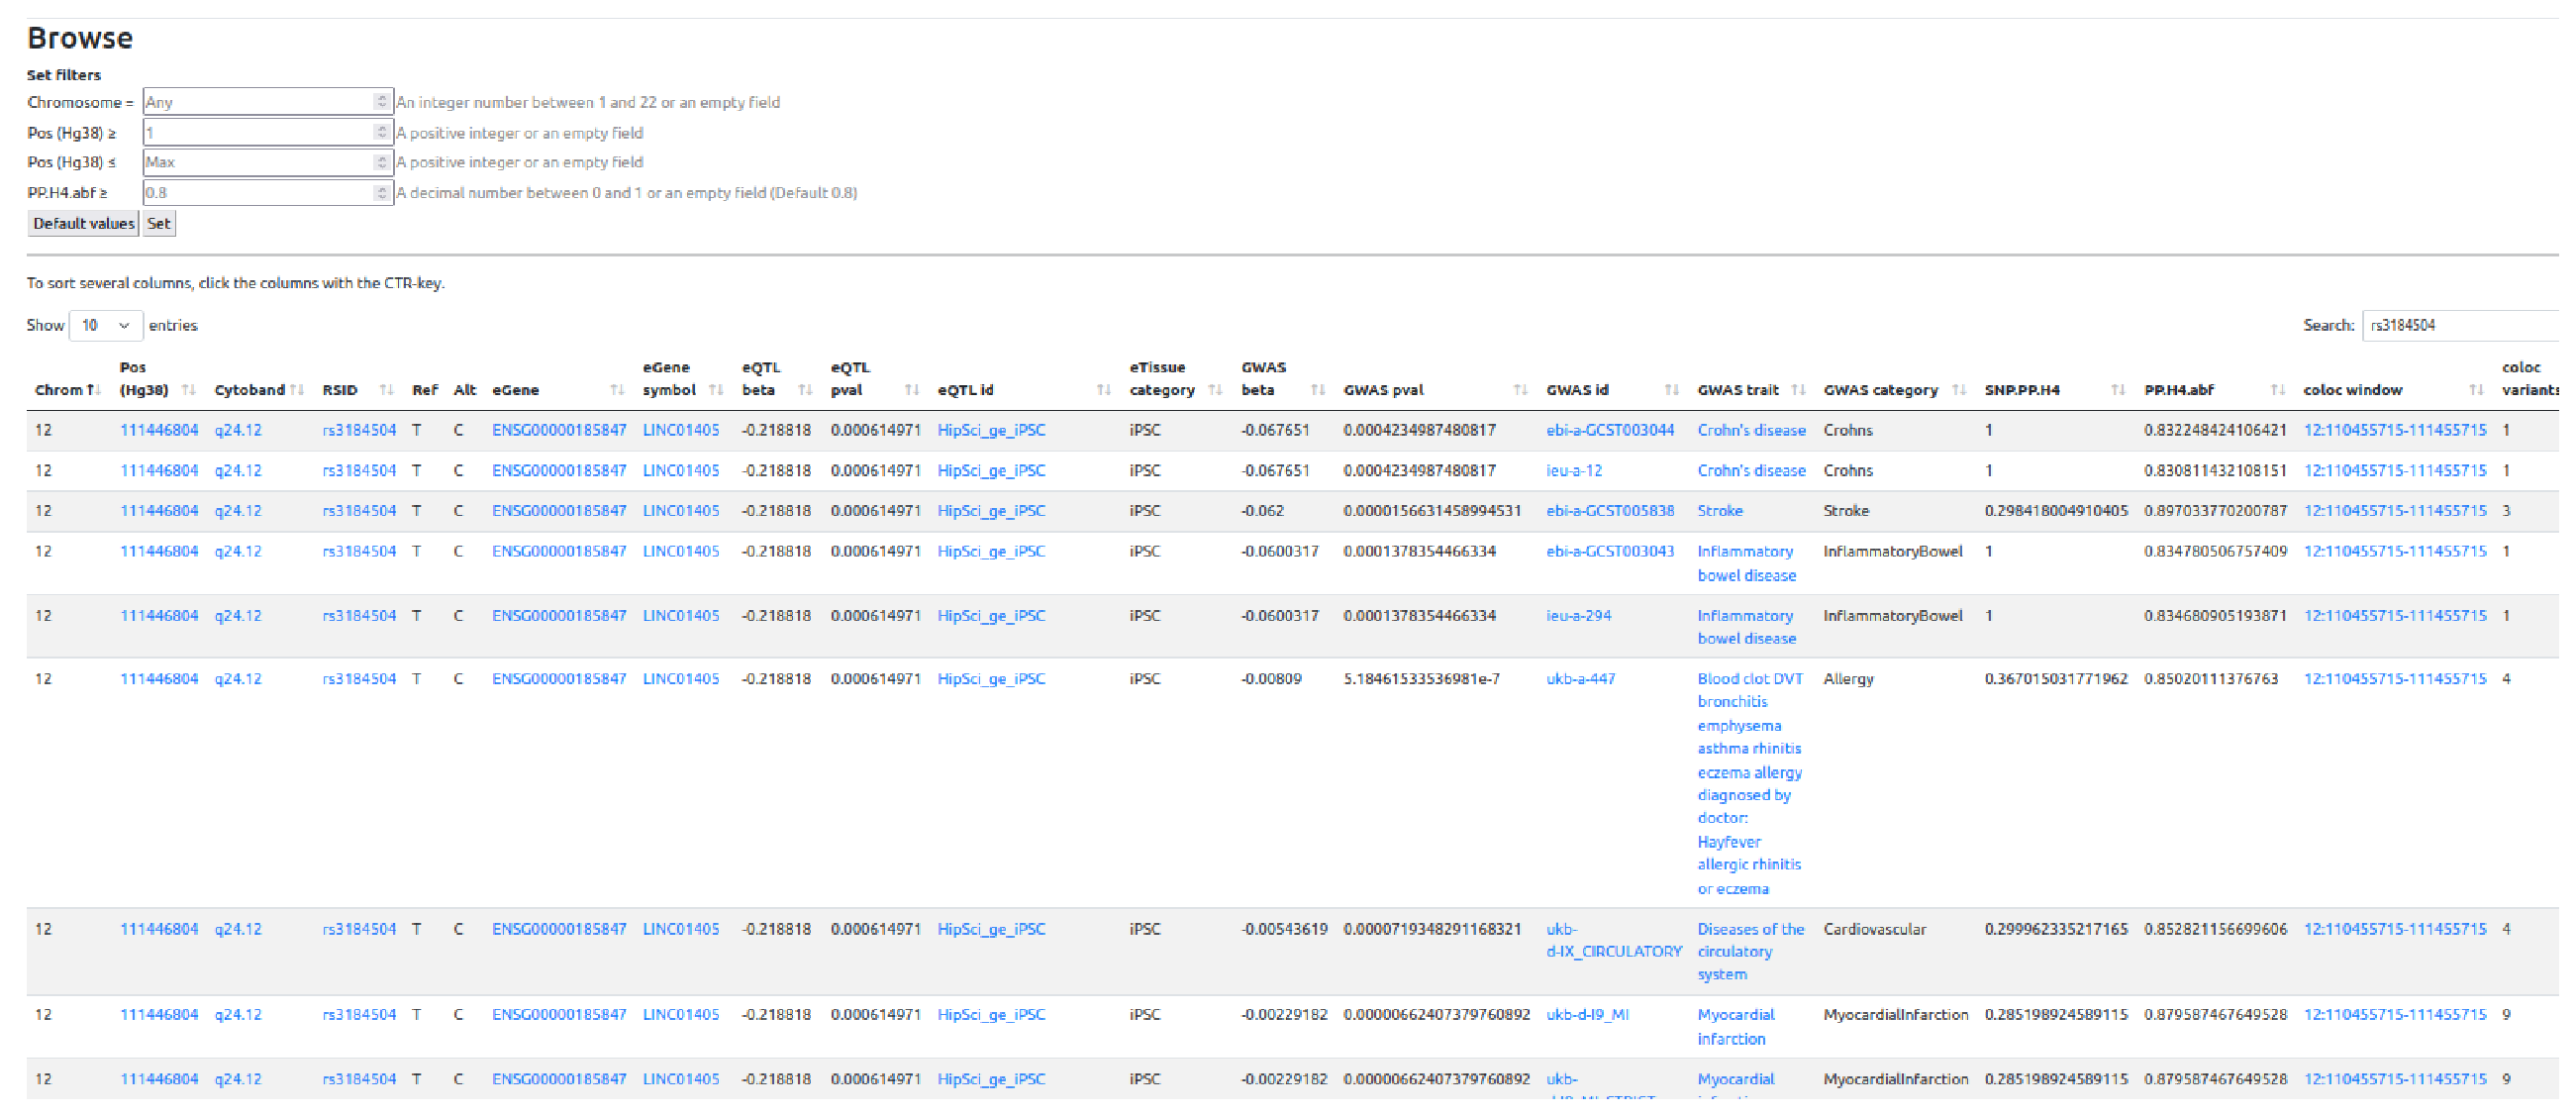
\includegraphics[width=0.6\textwidth]{/home/gonzalez/Repositories/gwas2eqtl_pleiotropy/poster_eccb22_barcelona/img/web.eps}
%\end{figure}

\end{frame}

%%%%%%%%%%%%%%%%%%%%%%%%%%%%%%%%%%%%%%%%%%%%%%%%%%%%%%%%%%%%%%%%%%%%%%%%%%%%%%%%
\begin{frame}
\frametitle{Do GWAS traits cluster coherently?}

Distance between GWAS traits based on eQTL beta

\begin{figure}[!]
\includegraphics[width=0.5\textwidth]{/home/gonzalez/Repositories/gwas2eqtl_pleiotropy/out/gwas418/pval_5e-08/r2_0.1/kb_1000/window_1000000/plthtmp_disease_comorbidity_matrix.py/corr.png}
\end{figure}

Clustering coherent

\end{frame}

%%%%%%%%%%%%%%%%%%%%%%%%%%%%%%%%%%%%%%%%%%%%%%%%%%%%%%%%%%%%%%%%%%%%%%%%%%%%%%%
%\begin{frame}
%\frametitle{Which are the most pleiotropic variants?}

%\begin{table}[!tbp]
%\centering
%\scriptsize
%\hline
%\csvreader[separator=tab,
%tabular=ccrrp{0.4\textwidth},
%head,
%table head=\bfseries Chrom. & \bfseries Cytoband & \bfseries Pos (hg38) & \bfseries Variant & \bfseries GWAS Categories\\\hline,
%]{/home/gonzalez/Repositories/gwas2eqtl_pleiotropy/out/gwas418/pval_5e-08/r2_0.1/kb_1000/window_1000000/cmpt_count_per_rsid.py/count_per_rsid_gwas_ms.tsv}{}% use head of csv as column names
%{\csvcoli\ & \csvcolii\ & \csvcoliii\ & \csvcoliv & \csvcolv}% specify your coloumns here
%\hline
%%
%\vspace{15pt}
%%
%\caption{Colocalized eQTL/GWAS variants involved in 5 or more GWAS categories. Genomic coordinates are given for the hg38 assembly. }\label{tab:pleitropic_variants}
%\end{table}

%\end{frame}


%%%%%%%%%%%%%%%%%%%%%%%%%%%%%%%%%%%%%%%%%%%%%%%%%%%%%%%%%%%%%%%%%%%%%%%%%%%%%%%%
\begin{frame}
\frametitle{How are pleiotropic variants distributed?}

\begin{columns}
\begin{column}{0.32\textwidth}
    \begin{center}
\includegraphics[width=\textwidth]{/home/gonzalez/Repositories/gwas2eqtl_pleiotropy/out/gwas418/pval_5e-08/r2_0.1/kb_1000/window_1000000/pltsctr_x_per_rsid_y_gwas.py/count_per_rsid_chr19_start48668049_end48756272_categories8.png}
     \end{center}
\end{column}
\begin{column}{0.32\textwidth}
    \begin{center}
\includegraphics[width=\textwidth]{/home/gonzalez/Repositories/gwas2eqtl_pleiotropy/out/gwas418/pval_5e-08/r2_0.1/kb_1000/window_1000000/pltsctr_x_per_rsid_y_egene.py/count_per_rsid_chr19_start48668049_end48756272_categories8.png}
     \end{center}
\end{column}
\begin{column}{0.32\textwidth}
    \begin{center}
\includegraphics[width=\textwidth]{/home/gonzalez/Repositories/gwas2eqtl_pleiotropy/out/gwas418/pval_5e-08/r2_0.1/kb_1000/window_1000000/pltsctr_x_per_rsid_y_egene.py/count_per_rsid_chr19_start48668049_end48756272_categories8.png}
     \end{center}
\end{column}
\end{columns}
%
\vfill
%
Neighboring variants show similar pleiotropy.

\end{frame}

%%%%%%%%%%%%%%%%%%%%%%%%%%%%%%%%%%%%%%%%%%%%%%%%%%%%%%%%%%%%%%%%%%%%%%%%%%%%%%%%
\begin{frame}
\frametitle{Where are the pleiotropic variants?$^1$}

    \begin{center}
\includegraphics[width=0.8\textwidth]{/home/gonzalez/Repositories/gwas2eqtl_pleiotropy/out/gwas418/pval_5e-08/r2_0.1/kb_1000/window_1000000/pltbar_vep_consequence.py/vep.png}
     \end{center}
varianb
\let\thefootnote\relax\footnotetext{$^1$https://www.ensembl.org/vep}
     
\end{frame}

%%%%%%%%%%%%%%%%%%%%%%%%%%%%%%%%%%%%%%%%%%%%%%%%%%%%%%%%%%%%%%%%%%%%%%%%%%%%%%%%
\begin{frame}
\frametitle{Do pleiotropic variants associate to more egenes?}

\begin{columns}
\begin{column}{0.5\textwidth}
    \begin{center}
\includegraphics[width=0.7\textwidth]{/home/gonzalez/Repositories/gwas2eqtl_pleiotropy/presentation_gold2022_paris/fig/model_pleio_egenes.png}
     \end{center}
\end{column}
\begin{column}{0.5\textwidth}  %%<--- here
    \begin{center}
\includegraphics[width=\textwidth]{/home/gonzalez/Repositories/gwas2eqtl_pleiotropy/out/gwas418/pval_5e-08/r2_0.1/kb_1000/window_1000000/pltbar_x_per_variant_etissue_y_egene.py/plt.png}
     \end{center}
\end{column}
\end{columns}

\end{frame}

%%%%%%%%%%%%%%%%%%%%%%%%%%%%%%%%%%%%%%%%%%%%%%%%%%%%%%%%%%%%%%%%%%%%%%%%%%%%%%%%
\begin{frame}
\frametitle{Do pleiotropic variants associate to more etissues?}

\begin{columns}
\begin{column}{0.5\textwidth}
    \begin{center}
\includegraphics[width=0.7\textwidth]{/home/gonzalez/Repositories/gwas2eqtl_pleiotropy/presentation_gold2022_paris/fig/model_pleio_etissues.png}
     \end{center}
\end{column}
\begin{column}{0.5\textwidth}  %%<--- here
    \begin{center}
\includegraphics[width=\textwidth]{/home/gonzalez/Repositories/gwas2eqtl_pleiotropy/out/gwas418/pval_5e-08/r2_0.1/kb_1000/window_1000000/pltbar_x_per_variant_egene_y_etissue.py/plt.png}
     \end{center}
\end{column}
\end{columns}

\end{frame}

%%%%%%%%%%%%%%%%%%%%%%%%%%%%%%%%%%%%%%%%%%%%%%%%%%%%%%%%%%%%%%%%%%%%%%%%%%%%%%%%
\begin{frame}
\frametitle{Do pleiotropic variants associate to more traits (after fixing egene-etissue)?}

\begin{columns}
\begin{column}{0.5\textwidth}
    \begin{center}
\includegraphics[width=0.7\textwidth]{/home/gonzalez/Repositories/gwas2eqtl_pleiotropy/presentation_gold2022_paris/fig/model_pleio_gwas.png}
     \end{center}
\end{column}
\begin{column}{0.5\textwidth}  %%<--- here
    \begin{center}
\includegraphics[width=\textwidth]{/home/gonzalez/Repositories/gwas2eqtl_pleiotropy/out/gwas418/pval_5e-08/r2_0.1/kb_1000/window_1000000/pltbar_x_per_variant_egene_etissue_y_gwas.py/plt.png}
     \end{center}
\end{column}
\end{columns}

\end{frame}

%%%%%%%%%%%%%%%%%%%%%%%%%%%%%%%%%%%%%%%%%%%%%%%%%%%%%%%%%%%%%%%%%%%%%%%%%%%%%%%%
\begin{frame}
\frametitle{Do pleiotropic variants bind more transcription factors?$^1$}

\begin{columns}
\begin{column}{0.5\textwidth}
    \begin{center}
\includegraphics[width=\textwidth]{/home/gonzalez/Repositories/gwas2eqtl_pleiotropy/out/gwas418/pval_5e-08/r2_0.1/kb_1000/window_1000000/pltbox_x_per_rsid_y_remapnr.py/bxplt_remaptf_per_rsid_flank_10.png}
     \end{center}
\end{column}
\begin{column}{0.5\textwidth}  %%<--- here
    \begin{center}
\includegraphics[width=\textwidth]{/home/gonzalez/Repositories/gwas2eqtl_pleiotropy/out/gwas418/pval_5e-08/r2_0.1/kb_1000/window_1000000/pltbar_x_per_variant_pleiotropy_y_remapcrm.py/remapcrm_flank10.png}
     \end{center}
\end{column}
\end{columns}

\end{frame}

\let\thefootnote\relax\footnotetext{$^1$https://remap.univ-amu.fr}

\section{Conclusions, perspective and acknowledgements} %%%%%%%%%%%%%%%%%%%%%%%%%%%%%%%%%%%%%%%%%%%%%%%%%%%%%%%%%%%%%%

%%%%%%%%%%%%%%%%%%%%%%%%%%%%%%%%%%%%%%%%%%%%%%%%%%%%%%%%%%%%%%%%%%%%%%%%%%%%%%%%
\begin{frame}
\frametitle{Conclusions}

Regulatory characteristics of pleiotropic variants
%
\begin{itemize}
\item Variant pleiotropy is correlated in regions
\item Enrichment of variants upstream (incl. 5'UTR) and downstream of genes (incl. 3'UTR)
\item Enrichment of transcription factor and CRM binding
\item Increased number of associated egenes and etissues
\end{itemize}
%
\vfill
%
Other outcomes of this study
%
\begin{itemize}
\item A large analysis of GWAS/eQTL colocalisations
\item A list of pleiotropic variants and regions
\end{itemize}

\end{frame}

%%%%%%%%%%%%%%%%%%%%%%%%%%%%%%%%%%%%%%%%%%%%%%%%%%%%%%%%%%%%%%%%%%%%%%%%%%%%%%%%
\begin{frame}
\frametitle{Perspectives}


\begin{itemize}
\item A web portail to share data
\item Causality of egenes on gwas (Looking for experts ;-) )
\end{itemize}

\end{frame}

%%%%%%%%%%%%%%%%%%%%%%%%%%%%%%%%%%%%%%%%%%%%%%%%%%%%%%%%%%%%%%%%%%%%%%%%%%%%%%%%
\begin{frame}
\frametitle{Acknowledgements}

\begin{itemize}
\item L\'eopoldine Lecerf (M1)
\item P Paul, P Rihet, M Michel, S Marquet, S Spicuglia
\end{itemize}
%
\vfill
%
Funding
%
\begin{itemize}
\item Institut Cancer et Immunologie (ICI)
\item Agence nationale de la recherche (ANR)
\item GOLD
\end{itemize}

\end{frame}

\end{document}


